% =====================================================================
%  第 4 章 §4.4 —— Maslov 指数与拉格朗日配边（含第 4 章章末评注）
%  页段：原书 p.163–186（PDF 173–196）
%  译者：tr06
% =====================================================================

% [原文 p.163]
定理 4.117 的实极化带有奇点，定理 4.87 不能原样适用。然而 Jeffrey–Weitsman [191] 证明了结论仍然成立。

\begin{theorem}{4.120}
  $\rank H^0\bigl(R(\Sigma,E);\cL^{\otimes k}\bigr) = \sharp\bigl(kf(R(\Sigma,E))\cap \Z^{3g-3}\bigr)$.
\end{theorem}

证明从略。式 (4.21) 的类似物可作为它的推论得到。

定理 4.117 的证明，除维数计算之外，对任意紧 Lie 群都成立。然而当 $\dim G\neq 3$ 时，$f$ 的纤维的维数不等于 $\dim R(\Sigma,E)$ 的一半，因而 $f$ 不是实极化。高仓树 [353] 考虑了既非实极化也非复极化的中间极化（intermediate polarization）这一概念，并证明了对于一般的 $G$，$\dim R(\Sigma,E)$ 具有这种极化。

定理 4.119 被 Andersen–Mattes–Reshetikhin [6], [7] 与 $R(\Sigma,E)$ 的形变量子化联系了起来。这些研究似乎以把 Chern–Simons 微扰理论（[27], [28], [217]）推广到带边 3 维流形为目的之一，目前仍在进行中。

\section{Maslov 指数与拉格朗日配边}

\takeaway{Maslov 指数是闭曲线到拉格朗日 Grassmann 流形的一种整值同伦不变量；本节把它推广为拉格朗日子流形在 $\pi_2(M,L)$ 上的不变量，并用 Thom–Pontryagin 式构造把拉格朗日（Legendre）配边半群算成同伦群。}

Maslov 指数是 Maslov 在偏微分方程的研究中发现的（[246]），它在超局部解析（micro local analysis）中发挥了重要作用。此后，它与拉格朗日配边研究的关联、与伪全纯曲线的关联等相继被发现，人们由此认清它是辛几何中的一个重要概念。

在 $\C^n=\R^{2n}$ 上赋予通常的辛结构 $\omega_{\C^n}$。令 $\operatorname{Gr}(n;\R^{2n})$ 为它的 $n$ 维线性子空间全体，$\operatorname{Gr}'(n;\R^{2n})$ 为带 $\omega_{\C^n}$ 所定定向的 $n$ 维线性子空间全体。它们称为 Grassmann 流形（Grassmannian manifold）。存在二重覆盖映射 $\operatorname{Gr}'(n;\R^{2n})\to\operatorname{Gr}(n;\R^{2n})$。

\begin{definition}{4.121}
  令 $\Lag_n$ 为 $\operatorname{Gr}(n;\R^{2n})$ 中使 $\omega_{\C^n}$ 在其上消失的元素 $L$ 全体，令 $\Lag'_n$ 为 $\operatorname{Gr}'(n;\R^{2n})$ 中使 $\omega_{\C^n}$ 在其上消失的元素 $L$ 全体。它们称为拉格朗日 Grassmann 流形（Lagrangian Grassmannian manifold）。
\end{definition}

% [原文 p.164]
$\pi_1(\operatorname{Gr}(n;\R^{2n}))=\Z_2$，其生成元对应定向。换言之，第 1 Stiefel–Whitney 类（1st Stiefel-Whitney class）给出同构 $w^1\colon\pi_1(\operatorname{Gr}(n;\R^{2n}))\simeq\Z_2$（$w^1$ 所定的二重覆盖正是 $\operatorname{Gr}'(n;\R^{2n})$）。

\begin{theorem}{4.122}
  $\pi_1(\Lag_n)=\Z$。并且存在交换图式 (4.26)。
  \begin{equation}
    \begin{array}{ccc}
      \Z=\pi_1(\Lag'_n) & \longrightarrow & \pi_1(\operatorname{Gr}'(n;\R^{2n}))=0 \\[6pt]
      \big\downarrow{\scriptstyle\times 2} & \circlearrowleft & \big\downarrow \\[6pt]
      \Z=\pi_1(\Lag_n) & \longrightarrow & \pi_1(\operatorname{Gr}(n;\R^{2n}))=\Z_2
    \end{array}
    \tag{4.26}
  \end{equation}
\end{theorem}

由定理 4.122 还可知道 $\pi_1(\Lag'_n)=\Z$，且存在二重覆盖映射 $\Lag'_n\to\Lag_n$。

\begin{definition}{4.123}
  定理 4.122 中的同构 $\in\Hom(\pi_1(\Lag_n),\Z)\simeq H^1(\Lag_n;\Z)$ 称为普遍 Maslov 类（universal Maslov class）。

  又，对闭曲线 $\gamma\colon S^1\to\Lag_n$，定理 4.122 的同构所对应的整数称为 $\gamma$ 的 Maslov 指数（Maslov index）。
\end{definition}

% [Tutor Note: 图式 (4.26) 左列的竖直箭头是 $\times 2$：二重覆盖 $\Lag'_n\to\Lag_n$ 的次数为 2，故 $\pi_1(\Lag'_n)=\Z$ 到 $\pi_1(\Lag_n)=\Z$ 的诱导映射是乘 2。于是落在 $\Lag_n$ 里的闭曲线，其 Maslov 指数必为偶数；奇数值只有在 $\Lag'_n$ 上才出现。]

\begin{proof}[定理 4.122 的证明]
  用 $Sp(n)$ 表示保持 $\R^{2n}$ 上 $\omega_{\C^n}$ 的线性变换全体（称为辛群）。辛群作用于 $\Lag_n$, $\Lag'_n$。令
  \[
    Sp(n)_0=\{g\in Sp(n)\mid g\R^n=\R^n\},
  \]
  \[
    Sp(n)_{00}=\{g\in Sp(n)\mid g\R^n=\R^n,\ g\ \text{在}\ \R^n\ \text{上的作用保持定向}\}.
  \]

  \begin{lemma}{4.124}
    $Sp(n)$ 在 $\Lag_n$, $\Lag'_n$ 上的作用是传递的。
  \end{lemma}

  证明留给读者。由引理得
  \[
    \Lag_n=Sp(n)/Sp(n)_0,\qquad \Lag'_n=Sp(n)/Sp(n)_{00}.
  \]
  注意 $U(n)$（酉群）是 $Sp(n)$ 的子群。此时有

  \begin{lemma}{4.125}
    $U(n)\subset Sp(n)$ 是同伦等价映射。
  \end{lemma}

  证明留给读者（用矩阵的极分解）。于是

  % [原文 p.165]
  \[
    U(n)\cap Sp(n)_0=O(n),\qquad U(n)\cap Sp(n)_{00}=SO(n).
  \]
  由此得到下述命题。

  \begin{proposition}{4.126}
    $\Lag_n$ 与 $U(n)/O(n)$ 同伦等价，$\Lag'_n$ 与 $U(n)/SO(n)$ 同伦等价。
  \end{proposition}

  由同伦正合列
  \[
    \pi_1(O(n))\to\pi_1(U(n))\to\pi_1(U(n)/O(n))\to\pi_0(O(n))\to 1
  \]
  以及同构 $\pi_1(O(n))=\Z_2$, $\pi_1(U(n))=\Z$，可知 $\pi_1(\Lag_n)=\Z$。又，$\pi_0(O(n))=\Z_2$ 的非零元表示 $w^1$，故存在满射 $\pi_1(\Lag_n)=\pi_1(U(n)/O(n))\to\pi_0(O(n))$，它使图式 (4.26) 成为交换图。
\end{proof}

由命题 4.126，$\Lag_n$, $\Lag'_n$ 的高次上同调也可算出。这里只写下答案（证明见 [49], [369]）。

\begin{theorem}{4.127}
  \[
    H^*(\Lag_{2n};\Q)\simeq H^*(\Lag_{2n-1};\Q)\simeq H^*(S^1\times S^5\times\cdots\times S^{4n-3};\Q),
  \]
  \[
    H^*(\Lag'_{2n-1};\Q)\simeq H^*(S^1\times S^5\times\cdots\times S^{4n-3};\Q),
  \]
  \[
    H^*(\Lag'_{2n};\Q)\simeq H^*(S^1\times S^5\times\cdots\times S^{4n-3}\times S^{2n};\Q).
  \]
\end{theorem}

下面说明 Maslov 指数更具体的计算方法。令 $\Lag_{n,0}$, $\Lag'_{n,0}$ 为分别与 $\sqrt{-1}\,\R^n$ 横截的 $\Lag_n$, $\Lag'_n$ 的元素全体。

\begin{lemma*}{4.128}
  $\Lag_{n,0}$, $\Lag'_{n,0}$ 可缩。
\end{lemma*}

\begin{proof}
  $\Lag_{n,0}$ 的元素 $L$ 可看作线性映射 $\psi_L\colon\R^n\to\sqrt{-1}\,\R^n$。对 $t\in\R$，$t\psi_L$ 仍对应 $\Lag_{n,0}$ 的一个元素。把它记作 $f_t(L)$。因 $f_0(L)=\R^n$，故 $f$ 是把 $\Lag_{n,0}$ 收缩到一点的同伦。$\Lag'_{n,0}$ 的情形证明相同。
\end{proof}

\begin{proposition*}{4.129}
  $\Lag_n-\Lag_{n,0}$, $\Lag'_n-\Lag'_{n,0}$ 是表示普遍 Maslov 类之 Poincaré 对偶的闭链。
\end{proposition*}

\begin{proof}
  容易看出 $\Lag_n-\Lag_{n,0}$ 在 $\Lag_n$ 中余维数为 1。于是由引理 4.128 即得命题 4.129。
\end{proof}

由命题 4.129 可得闭曲线 $\gamma\colon S^1\to\Lag_n$ 的 Maslov 指数的计算方法。即：取 $\gamma$ 与 $\Lag_n-\Lag_{n,0}$ 横截，每当它横穿 $\Lag_n-\Lag_{n,0}$ 时给它 $\pm 1$，再求和即可。

% [原文 p.166]
符号 $\pm 1$ 的取法说明如下。把 $\C^n$ 看作 $\R^n$ 的余切丛 $T^*\R^n$。不过要把头歪一歪，令 $\sqrt{-1}\,\R^n$ 为零截面（也就是说，把实部方向当作纤维方向）。设 $L\in\Lag_n$。可设 $L$ 与 $\R^n$ 横截而不失一般性。考虑 $L$ 与 $\sqrt{-1}\,\R^n$ 不横截的情形。把 $L$ 看作 $T^*\R^n$ 的子集，则 $L$ 可看作 $\R^n$ 上某个闭微分 1 形式 $u$ 的图像。因 $L$ 是线性的，$u$ 是某个二次形式 $f$ 的 $\rd f$。当 $f$ 的特征值中有 0 时，$L$ 与 $\sqrt{-1}\,\R^n$ 就不再横截。

于是设 $L_t$ 是 $\Lag_n$ 中元素的一族，$L_0$ 与 $\sqrt{-1}\,\R^n$ 不横截。设 $L_t$ 是 $\rd f_t$ 的图像。此时，在 $f_0$ 附近 $f_t$ 的特征值有一个改变符号（这等于说，$L_t$ 与 $\Lag_n-\Lag_{n,0}$ 横截）。于是规定符号：特征值由负变正时取 $+1$，由正变负时取 $-1$。

下面定义辛流形 $(M,\omega_M)$ 的拉格朗日子流形 $L$ 的 Maslov 指数 $\mu\colon\pi_2(M,L)\to\Z$。设 $u\colon(D^2,\partial D^2)\to(M,L)$。取 $M$ 上与 $\omega_M$ 相容的近复结构 $J_M$。$D^2$ 上的复向量丛 $u^*TM$ 存在唯一的平凡化：
\begin{equation}
  u^*TM\simeq D^2\times\C^n \tag{4.27}
\end{equation}
把它写作 (4.27)。限制到 $\partial D^2$ 上，$z\in\partial D^2\mapsto T_{u(z)}L$ 借助同构 (4.27) 诱导出映射
\begin{equation}
  \partial D^2\longrightarrow\Lag_n. \tag{4.28}
\end{equation}

\begin{definition}{4.130}
  (4.28) 的 Maslov 指数称为 $[u]\in\pi_2(M,L)$ 的 Maslov 指数，记作 $\mu(u)$。
\end{definition}

(4.28) 的 Maslov 指数不依赖于近复结构、平凡化 (4.27) 以及 $[u]$ 的代表元的取法，这是显然的。（不依赖近复结构的取法，依据与辛结构相容的近复结构之集合连通（命题 2.25）。）

余切丛的情形可定义 $\mu\colon\pi_1(L)\to\Z$。先朴素地定义。设 $i\colon L\to T^*N$ 是拉格朗日浸入。移动 $i$，使以下所需的横截正则性

% [原文 p.167]
成立。设 $[\gamma]\in\pi_1(L)$。对 $x\in T^*N$，纤维方向的切向量全体构成 $T_xT^*N$ 的子空间 $F_x$。与说明 Maslov 指数计算方法时同样地定义 $\epsilon_i=\pm 1$。即：在 $\gamma(t_i)$ 的附近，把 $T^*M$ 与 $T^*\R^n$ 等同。不过要旋转 90 度，使 $T^*M$ 的纤维方向对应 $T^*\R^n$ 的 $\R^n$（零截面）的方向。把 $(\rd i)(T_tL)$ 看作二次形式 $f_t$ 的图像。依 $f_t$ 的特征值在 $t_i$ 附近是从负穿过 0 到正、还是从正穿过 0 到负，取 $\epsilon_i=1$ 或 $\epsilon_i=-1$。
\begin{equation}
  \mu(\gamma)=\sum_{i=1}^{m}\epsilon_i \tag{4.29}
\end{equation}
如此定义。

% [Tutor Note: 原书 p.167 这里两处写 $T^*M$，但它前面刚把底流形记为 $N$（$i\colon L\to T^*N$），$L$ 并不在 $T^*M$ 里。疑为笔误，应作 $T^*N$；正文照原书写，读者按 $N$ 理解即可。]

作为例子，试计算图 4.8 的情形（$\C=T^*\R^1$ 的拉格朗日子流形）（这里把 $y$ 轴方向看作纤维）。图 4.8(a) 中，纤维方向与 $(\rd i)(T_tL)$ 不横截的点有 2 个，而且在两点处 $(\rd i)(T_tL)$ 都是逆时针旋转的。故 $\pi_1(S^1)$ 的生成元的 Maslov 指数为 2。另一方面，图 4.8(b) 中，一侧（右侧）逆时针旋转，另一侧顺时针旋转。故 $\pi_1(S^1)$ 的生成元的 Maslov 指数为 0。

\begin{figure}[htbp]
  \centering
  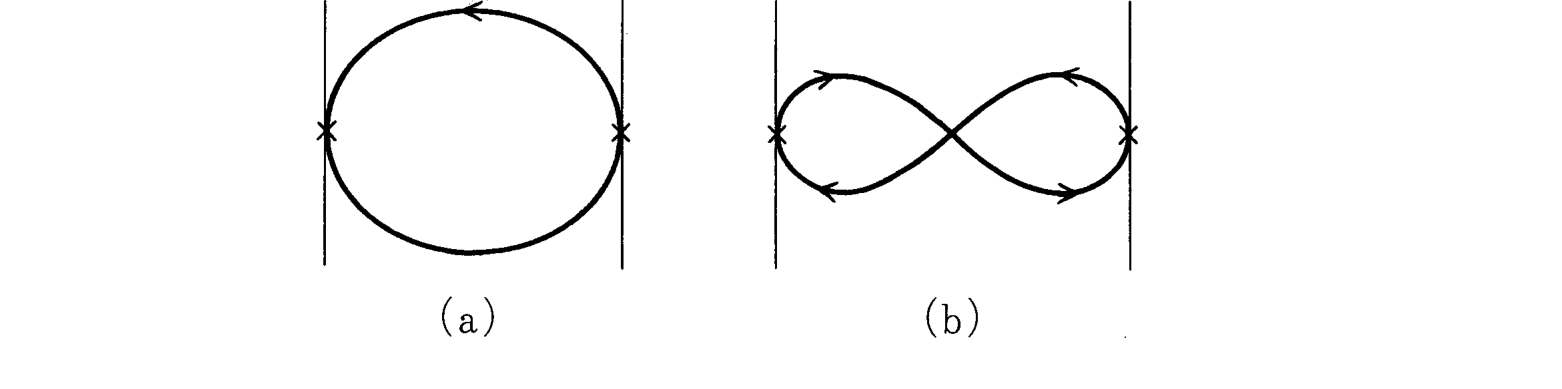
\includegraphics[width=0.62\textwidth]{figures/fig4.8.png}
  \figtitle{4.8}{Maslov 指数的计算（原书 p.167）}
\end{figure}

% [Tutor Note: 图 4.8 的两条竖直线是纤维方向（即 $\sqrt{-1}\,\R$ 的方向），曲线与竖直线交于两点，那里 $(\rd i)(T_tL)$ 与纤维方向不横截。Maslov 指数数的是这些交点的带号个数：绕一圈得 $2\times(+1)=2$ 对应 (a)，一正一负相消得 0 对应 (b)。注意这正好是 $\Lag_1-\Lag_{1,0}$ 的交点计数（命题 4.129）。]

下面再稍微抽象地看待这个定义。（我们还没有证明 (4.29) 只依赖于 $\gamma$ 的同伦类。）为此要用纤维丛的代数拓扑。首先，命题 4.126 可以改述如下。令 $\operatorname{Gr}(n;\C^m)$ 为 $\C^m$ 中 $n$ 维复子空间全体，$\operatorname{Gr}(n;\R^m)$ 为 $\R^m$ 中 $n$ 维实子空间全体，并把它们在 $m\to\infty$ 时的归纳极限记为 $\operatorname{Gr}^{\C}(n;\infty)$, $\operatorname{Gr}^{\R}(n;\infty)$。$\R^m$ 中的 $n$ 维实子空间与 $\C$ 作张量积，就决定了 $\C^m$ 中的 $n$ 维复子空间，故有映射 $\mathrm{comp}\colon\operatorname{Gr}^{\R}(n;\infty)\to\operatorname{Gr}^{\C}(n;\infty)$。

% [原文 p.168]
\begin{lemma*}{4.131}
  $\mathrm{comp}$ 的纤维与 $\Lag_n$ 同伦等价。
\end{lemma*}

\begin{proof}
  $\operatorname{Gr}^{\C}(n;\infty)$, $\operatorname{Gr}^{\R}(n;\infty)$ 分别与可缩空间除以 $U(n)$, $O(n)$ 所得的空间同伦等价。故纤维与 $U(n)/O(n)$ 同伦等价。于是由命题 4.126 即得引理 4.131。
\end{proof}

设有两个映射 $f_1\colon X\to\operatorname{Gr}^{\R}(n;\infty)$, $f_2\colon X\to\operatorname{Gr}^{\R}(n;\infty)$，满足 $\mathrm{comp}\circ f_1\sim\mathrm{comp}\circ f_2$（$\sim$ 表示同伦）。于是它们的“差” $f_1-f_2\in[X\to\Lag_n]$ 被确定（$[X\to Y]$ 表示 $X$ 到 $Y$ 的映射的同伦类全体）。$f_1-f_2$ 在把 $f_1$, $f_2$ 同伦地变动时不变。

上述事实由引理 4.131 导出，这是关于纤维丛（或纤维空间）的基本事实。参见代数拓扑教科书（[175], [346] 等）。

又，由向量丛的分类定理（参见 [175], [346] 等），切向量丛的分类映射 $\mathrm{cl}_{TN}\colon N\to\operatorname{Gr}^{\R}(n;\infty)$ 被确定。另一方面，$T^*N$ 上确定了近复结构，故切向量丛的分类映射 $\mathrm{cl}_{T^*N}\colon T^*N\to\operatorname{Gr}^{\C}(n;\infty)$ 被确定。$T^*N$ 的切向量丛作为复向量丛，与 $TN$ 经 $\pi\colon T^*N\to N$ 拉回后的复化同构。因此
\begin{equation}
  \mathrm{comp}\circ\mathrm{cl}_{TN}\circ\pi\sim\mathrm{cl}_{T^*N} \tag{4.30}
\end{equation}
另一方面，设 $i\colon L\to T^*N$ 是拉格朗日浸入。线性空间 $(\rd i)(T_{i(t)}L)$ 与 $J_{T^*N}\bigl((\rd i)(T_{i(t)}L)\bigr)$ 横截，故二者张成 $T_{i(t)}T^*N$。因此确定同构 $i^*T(T^*N)\simeq TL\otimes\C$。从而
\begin{equation}
  \mathrm{cl}_{T^*N}\circ i\sim\mathrm{comp}\circ\mathrm{cl}_L \tag{4.31}
\end{equation}
（$\mathrm{cl}_L\colon L\to\operatorname{Gr}(n;\infty)$ 是 $L$ 的切向量丛的分类映射）。由 (4.30), (4.31) 得 $\mathrm{comp}\circ\mathrm{cl}_{TN}\circ\pi\circ i\sim\mathrm{comp}\circ\mathrm{cl}_L$，即 $\mathrm{cl}_{TN}\circ\pi\circ i$ 与 $\mathrm{cl}_L$ 是同一映射 $L\to\operatorname{Gr}^{\C}(n;\infty)$ 的不同提升。因此
\begin{equation}
  \mathrm{cl}_{TN}\circ\pi\circ i-\mathrm{cl}_L\in[L\to\Lag_n] \tag{4.32}
\end{equation}
被确定。把这个同伦类记作 $\eta_L$。

\begin{definition}{4.132}
  $\eta_{L*}\colon\pi_1(L)\to\pi_1(\Lag_n)=\Z$ 称为 Maslov 指数。
\end{definition}

下面两个引理的证明作为习题。

% [原文 p.169]
\begin{lemma}{4.133}
  定义 4.132 的 Maslov 指数与 (4.29) 一致。
\end{lemma}

\begin{lemma}{4.134}
  下图式 (4.33) 交换。这里左侧的映射是定义 4.130 的 Maslov 指数，右侧的映射是定义 4.132 的 Maslov 指数。
  \begin{equation}
    \begin{array}{ccc}
      \pi_2(M,L) & \longrightarrow & \pi_1(L)\\[10pt]
      \searrow & & \swarrow\\[10pt]
      & \Z &
    \end{array}
    \tag{4.33}
  \end{equation}
\end{lemma}

引理 4.134 意味着：在余切丛的情形，定义 4.132 的 Maslov 指数在 $\pi_2(M)\to\pi_2(M,L)$ 的像上为 0。这一点也是下述命题 4.135 的推论。辛流形 $(M,\omega)$ 上，相容的近复结构在连续形变下唯一确定。故 $TM$ 上有唯一的复向量丛结构，故 Chern 类 $c^k(TM)$ 被确定。把它简记为 $c^k(M)$。

\begin{proposition}{4.135}
  令 $c^1\colon\pi_2(M)\to\Z$ 为 $u\mapsto\int_{S^2}u^*c^1(M)$，则图式 (4.34) 交换。
  \begin{equation}
    \begin{array}{ccc}
      \pi_2(M) & \longrightarrow & \pi_2(M,L)\\[10pt]
      \underset{\scriptstyle 2c^1}{\searrow} & & \swarrow\\[10pt]
      & \Z &
    \end{array}
    \tag{4.34}
  \end{equation}
\end{proposition}

% [Tutor Note: (4.34) 左侧斜箭头上的 $2c^1$ 中的因子 2 不要漏：把 $S^2$ 上的映射看作圆盘映射时，$\partial D^2$ 走的是赤道，故圆盘 Maslov 指数等于球面的 $\langle c^1,[S^2]\rangle$ 的两倍。这样 (4.34) 与引理 4.134 才对得上。]

\begin{remark}{4.136}
  (4.29) 的算法也可改述如下。取 $[\gamma]\in\pi_1(L)$，考虑 $\pi\circ\gamma\colon S^1\to N$。每当这个合成映射碰到焦集合 $\subset N$ 时就给 $\pm 1$。（准确地说，碰到与所考虑的分支无关的焦集合时什么也不给，即图 4.9 左侧的焦点那种情形。）其和就是 Maslov 指数。此时，所考虑的焦集合只需取余维数 1 的组成部分、即折痕即可。

  由 $\eta_L$ 决定的更一般的映射 $\eta_{L*}\colon H_k(L)\to H_k(\Lag_n)$ 要研究，就需要考虑余维数更高的拉格朗日奇点。拉格朗日奇点与这种“高次 Maslov 指数”之间的关系也有人研究（Vassilyev\footnote{Vassilyev 就是因纽结不变量而闻名的 Vassiliev 的同一人。这里的英文拼写依照 [376]。} [376] 等参见）。
\end{remark}

% [原文 p.170]
\begin{figure}[htbp]
  \centering
  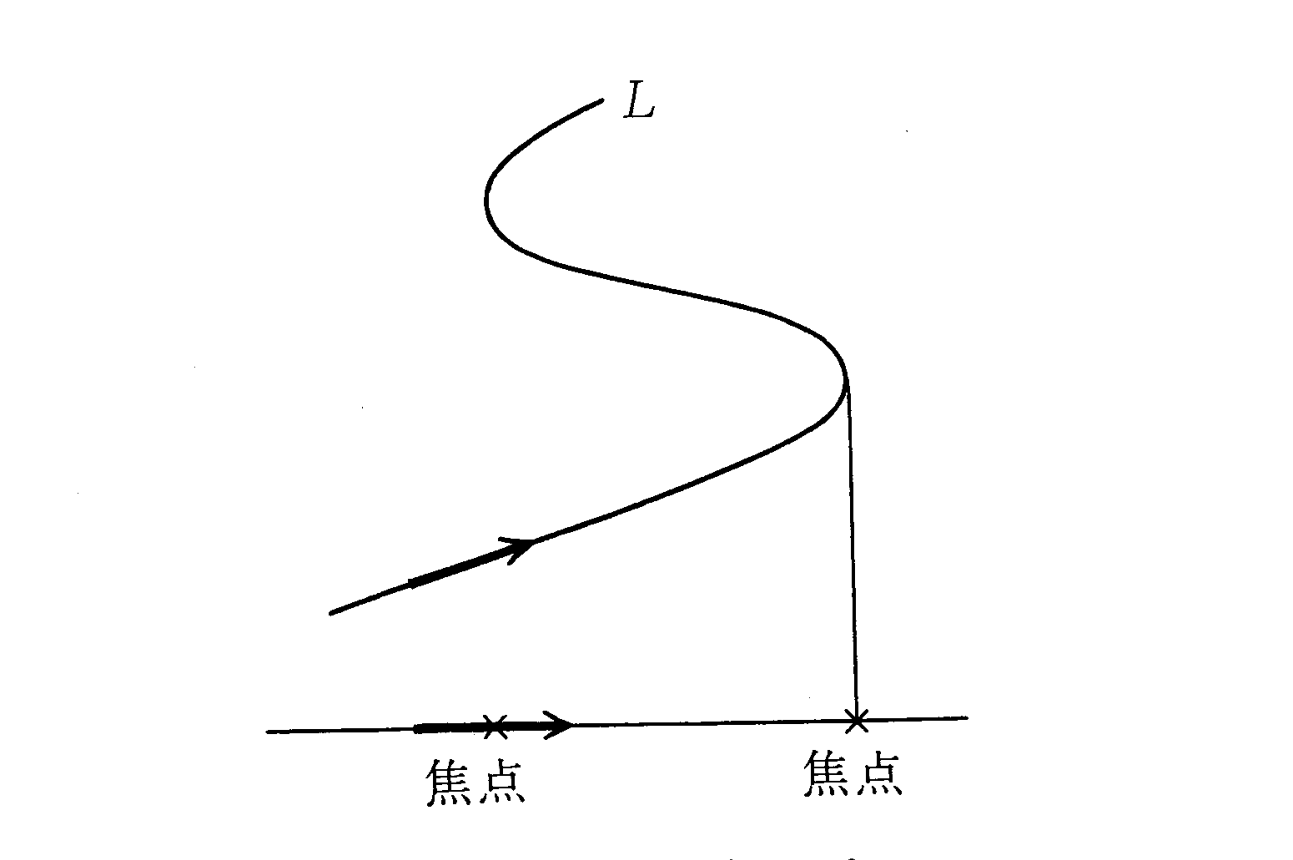
\includegraphics[width=0.52\textwidth]{figures/fig4.9.png}
  \figtitle{4.9}{什么也不给出（原书 p.170）}
\end{figure}

% [Tutor Note: 图 4.9 画的是 $S^1\to N$ 碰到焦集合的两种情形：左侧的焦点与所考虑的拉格朗日分支无关，不计符号；只有右侧那种顺着分支来的折痕才计入 $\pm 1$。这是“折痕 = 余维 1 的焦集合”这一说法的几何含义。]

Chern 类、Pontryagin 类（Pontrjagin class）、Stiefel–Whitney 类等示性类，在同调配边理论（cobordism theory）中起重要作用（参见 [1], [356] 等）。

Maslov 指数也与拉格朗日子流形的配边理论深刻相关。下面概述其梗概。拉格朗日配边的研究，一般认为始于 Arnold [12]。本书关于拉格朗日配边的讨论参考了 [376] 等（[23] 中写有配边群的计算等）。

先从配边概念的复习开始。

\begin{definition}{4.137}
  两个无边 $n$ 维紧流形 $M_1$, $M_2$ 称为配边（cobordant）的，是指存在带边的 $n+1$ 维紧流形 $W$，使 $\partial W=M_1\cup M_2$。

  当 $M_1$, $M_2$ 带定向时，它们称为定向配边（oriented cobordant）的，是指存在带定向的带边 $n+1$ 维紧流形 $W$，使 $\partial W=M_1\cup(-M_2)$。这里 $-M_2$ 指把 $M_2$ 的定向反转所得者。
\end{definition}

配边理论继 Pontrjagin、Rholin 的先驱性业绩之后由 Thom 创立，充当了微分拓扑学本身诞生的助产士（日语可读的解说有 [1], [356] 等）。以下要讲的拉格朗日配边理论，也用到了 Thom 等人的这些想法。

% [原文 p.171]
现在考虑 $n$ 维流形 $M_1$ 与 $M_2$ 的余切丛 $T^*M_1$ 与 $T^*M_2$。设 $i_1\colon L_1\to T^*M_1$, $i_2\colon L_2\to T^*M_2$ 是紧流形的拉格朗日浸入。设 $M_1$ 与 $M_2$ 配边，并按定义 4.137 的写法取 $\partial W=M_1\cup(-M_2)$。

\begin{definition}{4.138}
  $L_1$ 与 $L_2$ 在 $W$ 中拉格朗日配边（Lagrangian cobordant），是指存在 $n+1$ 维紧流形 $\hat L$ 与拉格朗日浸入 $i\colon\hat L\to T^*W$，满足下列条件：
  \begin{enumerate}[label=(\arabic*),leftmargin=2.6em,itemsep=2pt]
    \item $\partial\hat L=L_1\cup L_2$。
    \item $i^{-1}(M_1)=L_1$, $i^{-1}(M_2)=L_2$，且 $\hat L$ 与边界 $M_1$, $M_2$ 横截相交。
    \item $\pi\circ i|_{L_1}=i_1$, $\pi\circ i|_{L_2}=i_2$。这里 $\pi\colon T^*M|_{M_1}\to T^*M_1$ 是自然确定的映射。
  \end{enumerate}
  当 $L_1$, $L_2$ 可定向时，$L_1$ 与 $L_2$ 在 $W$ 中定向拉格朗日配边（oriented Lagrangian cobordant），是指 $\hat L$ 可定向，且把 (1) 换成 $\partial\hat L=L_1\cup(-L_2)$ 后上述条件满足。

  当 $M_1=M_2=M$, $W=M\times[0,1]$ 时，就简单地说 $L_1$ 与 $L_2$ 拉格朗日配边、定向拉格朗日配边。拉格朗日配边记作 $L_1\sim_{\mathrm{cob}}L_2$，定向拉格朗日配边记作 $L_1\sim_{\mathrm{o.cob}}L_2$（本书专用的记号）。
\end{definition}

% [Tutor Note: 条件 (3) 里的 $\pi$ 是 $T^*W$ 限制到边界 $M_1$ 上后向 $T^*M_1$ 的投影，原书 p.171 把它写成 $T^*M|_{M_1}\to T^*M_1$，其中 $M$ 应理解为 $W$；读到条件 (3) 时，直接把 $\pi$ 当作缩回余切丛的自然投影即可。]

以后本书只处理 $M_1=M_2=M$, $W=M\times[0,1]$ 的情形。

\begin{lemma*}{4.139}
  拉格朗日配边、定向拉格朗日配边都是等价关系。
\end{lemma*}

\begin{proof}
  $L_1\sim_{\mathrm{cob}}L_2\Rightarrow L_2\sim_{\mathrm{cob}}L_1$ 以及 $L\sim_{\mathrm{cob}}L$ 是显然的。下面证传递律 $L_1\sim_{\mathrm{cob}}L_2$, $L_2\sim_{\mathrm{cob}}L_3\Rightarrow L_1\sim_{\mathrm{cob}}L_3$。

  取 $i_{12}\colon\partial\hat L_{12}\to T^*(M\times[0,1])$, $i_{23}\colon\partial\hat L_{23}\to T^*(M\times[0,1])$，使它们满足 $\partial L_{12}=L_1\cup L_2$ 等定义中的条件。

  $T^*(M\times[0,1])=T^*M\times[0,1]\times\R$。在此等同之下，对 $x_{2;12}\in L_2\subset L_{12}$, $x_{2;23}\in L_2\subset L_{23}$，令 $i_{12}(x_{2;12})=(i_2(x),(1,g(x)))$, $i_{23}(x_{2;23})=(i_2(x),$ $(0,h(x)))$（$g$, $h$ 由此式定义）。若 $g\neq h$，则 $i_{12}$, $i_{23}$ 不能就这样粘合起来。

  % [原文 p.172]
  为处理这一点，取光滑函数 $\chi\colon[0,1]\to[0,1]$ 满足
  \[
    \chi(t)=
    \begin{cases}
      0, & t<2/5\ \text{时},\\
      1, & t>3/5\ \text{时}.
    \end{cases}
  \]
  对 $x=(y,t)\in T^*M\times[0,1]$，记 $\tau_1(x)=(y,t/3)$, $\tau_2(x)=(y,(t+2)/3)$。令 $L=L_{12}\cup(L_2\times[0,1])\cup L_{23}$，并按下列式子定义 $I\colon L\to T^*M\times[0,1]$：
  \[
    i(x)=
    \begin{cases}
      \tau_1\circ i_{12}(x), & x\in L_{12}\ \text{时},\\
      \bigl(i_2(y),(t+1)/3,(1-\chi(t))g(x)+\chi(t)h(y)\bigr), & x=(y,t)\in L_2\times[0,1]\ \text{时},\\
      \tau_2\circ i_{23}(x), & x\in L_{23}\ \text{时}.
    \end{cases}
  \]
  $(L,i)$ 给出 $L_1$ 与 $L_3$ 的拉格朗日配边，这是显然的。定向的情形也相同。
\end{proof}

下面考虑 Legendre 子流形的情形。在此之前先作一个重要的注意。

\begin{remark}{4.140}
  Legendre 子流形是 $2n+1$ 维流形中的 $n$ 维子流形。由 Whitney 定理，当存在从 $n$ 维流形 $N$ 到 $2n+1$ 维流形 $M$ 的映射时，稍加移动就能把它变成嵌入（参见 [356] 等）。若原来的映射是 Legendre 浸入，那么稍加移动即可使其成为 Legendre 嵌入，这一点（用引理 4.23）也不难证明。因此，为了配边理论等目的，不考虑 Legendre 浸入而只限于 Legendre 子流形，也不会失去什么。

  拉格朗日子流形的情形则不同。当存在从 $n$ 维流形到 $2n$ 维流形的映射时，总可以用浸入去逼近它。但用嵌入去逼近则不可能（考虑 $\R^2$ 中的 $S^1$ 即可明白）。不做逼近，而是在（保持浸入这一性质的前提下）大幅移动，看能否变成嵌入——这是微分拓扑学的基本问题

% [原文 p.173]
；而 $n>2$ 时，对 $\R^{2n}$ 中的 $n$ 维流形这一问题可以做到，这同样属于 Whitney 定理（[390]）。这个定理的证明与 $2n+1$ 的情形不同，用到了整体方法，即 Whitney 技巧\footnote{[258], [356] 中有解说。}。因此，拉格朗日嵌入与拉格朗日浸入的差别是重大的。在 §5.4 将看到不能作为拉格朗日子流形嵌入、却能浸入的流形之例。
\end{remark}

拉格朗日配边也可以考虑拉格朗日子流形的情形。（此时，无论把 $L_{12}$ 看作拉格朗日子流形还是看作拉格朗日浸入，结果由后面要讲的引理 4.145 是相同的。）拉格朗日浸入的配边类全体，一般认为与拉格朗日嵌入的配边类全体不同。

又，考虑 $T^*M\times\R$ 这一接触流形（引理 4.29），设 $L_1$, $L_2$ 为其紧 Legendre 子流形。把余切丛 $T^*(M\times[0,1])$ 限制到 $M\times\{0\}$ 及 $M\times\{1\}$ 上，并与 $T^*M\times\R$ 等同。

\begin{definition}{4.141}
  $L_1$ 与 $L_2$ Legendre 配边（Legendrian cobordant），是指存在 $T^*(M\times[0,1])$ 的紧拉格朗日子流形 $L_{12}$，它与边界 $\partial T^*(M\times[0,1])$ 横截相交，且在上述等同下 $L_{12}\cap\partial T^*(M\times[0,1])=L_1\cup L_2$。

  定向 Legendre 配边的定义也相同。
\end{definition}

容易看出 Legendre 配边是等价关系。

拉格朗日配边在非余切丛的情形该如何考虑，笔者不学无术，并不知道；但 Legendre 配边的定义可以容易地推广。设 $N$ 为接触流形，$N\times\R$ 为其辛化（定义 4.43）。设 $L_1$, $L_2$ 为 $N$ 的（紧）Legendre 子流形。

\begin{definition}{4.142}
  $L_1$, $L_2$ Legendre 配边，是指存在 $N\times[0,1]$ 的（紧）拉格朗日子流形 $L$，$L$ 与 $\partial(N\times[0,1])$ 横截相交，且满足 $L\cap(N\times\{0\})=L_1$, $L\cap(N\times\{1\})=L_2$。定向 Legendre 配边也相同。
\end{definition}

Legendre 配边在本书中也记作 $L_1\sim_{\mathrm{cob}}L_2$, $L_1\sim_{\mathrm{o.cob}}L_2$ 等。

% [原文 p.174]
辛化上的辛形式是 $e^t(\rd t\wedge\theta+\rd\theta)$，故对 Legendre 子流形 $L_1$，$L=L_1\times\R$ 是拉格朗日子流形。又，$N\times\R\to N\times\R$, $(x,t)\mapsto(x,-t)$ 不是辛同胚，却把拉格朗日子流形移到拉格朗日子流形。注意到这一点，便知 Legendre 配边是等价关系。

当 $N$ 有两个 Legendre 子流形 $L$, $L'$ 时，可稍作移动（不改变 Legendre 配边类），使这两者互不相交。

\begin{lemma*}{4.143}
  和 $L\cup L'$ 的 Legendre 配边类，只依赖于 $L$ 的 Legendre 配边类与 $L'$ 的 Legendre 配边类。
\end{lemma*}

\begin{proof}
  设 $L_1\sim_{\mathrm{cob}}L_2$，$L_{12}\subset N\times[0,1]$ 为给出配边的拉格朗日子流形。一般 $L_{12}$ 与 $L'\times[0,1]$ 会相交，故取二者之和便得到拉格朗日浸入。但是，做下面要讲的拉格朗日子流形手术，就能在不改变边界的前提下把它换成嵌入的拉格朗日子流形（引理 4.145）。因此 $L_1\cup L'\sim_{\mathrm{cob}}L_2\cup L'$。
\end{proof}

关于拉格朗日子流形的手术（Lagrange surgery），这里只稍作叙述。详见 [307]。这是局部操作，故只考虑 $\C^n$ 中的拉格朗日子流形就足够了。设 $\C^n$ 中有两个在原点横截相交的拉格朗日子流形。考虑 $L_a=\R^n$ 与 $L_b=\sqrt{-1}\,\R^n$ 的情形就足够了。把 $\C^n$ 看作 $T^*\R^n$（以 $\sqrt{-1}\,\R^n$ 为纤维方向）。令 $f\colon\R^n\to\R$ 为
\[
  f_\epsilon(x)=
  \begin{cases}
    0, & |x|>1\ \text{时},\\
    \epsilon\log|x|, & |x|<1/2\ \text{时}.
  \end{cases}
\]
$\rd f_\epsilon$ 的图像 $\mathrm{Graph}(\rd f_\epsilon)$ 是 $\C^n$ 的拉格朗日流形。它包含 $L_a$ 去掉某个紧集后所得者。把 $\mathrm{Graph}(\rd f_\epsilon)$ 稍作改变，使它也包含 $L_b$ 去掉某个紧集后所得者。

$\tau\colon\C^n\to\C^n$ 定义为 $z\mapsto\operatorname{Re}z+\sqrt{-1}\operatorname{Im}z$（即关于集合 $\operatorname{Re}z=\operatorname{Im}z$ 的折返）

% [Tutor Note: 原书 p.174 把 $\tau$ 写成 $z\mapsto\operatorname{Re}z+\sqrt{-1}\operatorname{Im}z$，这实际是恒等映射，与紧随其后的“关于 $\operatorname{Re}z=\operatorname{Im}z$ 的折返”不符，疑为笔误；按折返的含义应为 $z\mapsto\operatorname{Im}z+\sqrt{-1}\operatorname{Re}z$。正文照原书抄录，此处按折返理解。]

% [原文 p.175]
。$\epsilon\rd\log|x|$ 的图像关于 $\tau$ 不变。令 $V=\{z\in\C^n\mid |\operatorname{Im}z|\leqq|\operatorname{Re}z|\}$，并令
\[
  L=\bigl(V\cap\mathrm{Graph}(\rd f_\epsilon)\bigr)\cup\tau\bigl(V\cap\mathrm{Graph}(\rd f_\epsilon)\bigr).
\]
下述性质是显然的。

\begin{lemma}{4.144}
  $L$ 是光滑的拉格朗日子流形。$L$ 去掉某个紧集后所得者，与 $L_a\cup L_b$ 去掉某个紧集后所得者一致。
\end{lemma}

\begin{figure}[htbp]
  \centering
  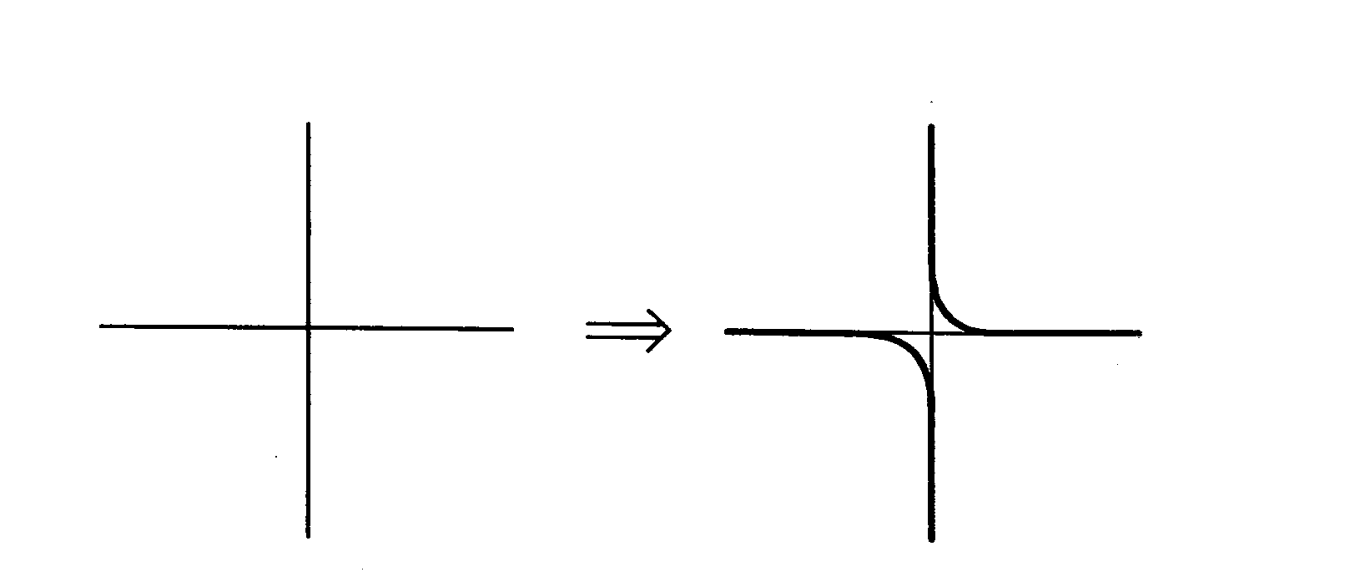
\includegraphics[width=0.56\textwidth]{figures/fig4.10.png}
  \figtitle{4.10}{拉格朗日子流形的手术（原书 p.175）}
\end{figure}

以上操作在自交的各点进行，便得到下述引理。

\begin{lemma}{4.145}
  设 $i\colon L\to M$ 是带边的拉格朗日浸入，且 $i$ 在 $\partial L$ 上是嵌入。则存在 $M$ 的嵌入拉格朗日子流形 $L'$，使 $\partial L'=\partial L$。并且，对 $i(L)$ 的任意小邻域，都能取到含于其中的 $L'$；又 $L$ 与 $L'$ 在 $\partial L$, $\partial L'$ 的邻域上一致。
\end{lemma}

以上便定义了和 $\cup$。$\cup$ 定义了半群结构。

\begin{definition}{4.146}
  在接触流形 $N$ 的 Legendre 子流形的配边类全体上，以 $\cup$ 求和所得者记作 $\cL_{uo}(N)$，称为非定向 Legendre bordism 半群。

  $T^*M$ 的拉格朗日浸入的配边类全体同样构成半群。记作 $\cL_{uo}(M)$，称为非定向拉格朗日 bordism 半群。

  分别在两者中考虑带定向的 Legendre（拉格朗日）子流形（浸入），并取其定向配边类，所得者记作 $\cL(N)$, $\cL(M)$。它们称为 Legendre bordism 半群、拉格朗日 bordism 半群。
\end{definition}

% [原文 p.176]
若要得到群，考虑 Grothendieck 群（K 群）即可。但 $T^*\R^n\times\R$ 的情形自动成为群。

\begin{lemma*}{4.147}
  $\cL(T^*\R^n\times\R)$ 是群。
\end{lemma*}

\begin{proof}
  设 $T^*\R^n$ 的坐标为 $x_i,y_i$, $i=1,\ldots,n$，$\R$ 的坐标为 $x_0$。设 $T^*(\R^n\times\R)$ 的坐标为 $x_i,y_i$, $i=0,\ldots,n$。这是 Darboux 坐标。可设 $L$ 含于 $T^*\R^n\times\R_+$ 之中。设 $r_\theta$ 为 $\R^2$ 的角度 $\theta$ 的旋转。把 $\R^2$ 看作第 0 与第 1 坐标，并把 $r_\theta$ 看作 $\R^{n+1}$ 的微分同胚（用同一记号）。于是 $r_\theta$ 诱导出 $T^*(\R^n\times\R)$ 的辛同胚，这也用同一记号书写。令 $\hat L=\bigcup_{\theta\in[0,\pi]}r_\theta(L)$，则它含于 $T^*\R^n\times\R^2_+$ 中，并给出 $L\cup(-r_\pi(L))$ 与空集之间的 Legendre 配边。因此 $-r_\pi(L)$ 是 $L$ 的逆元。其实 $-r_\pi(L)$ 与 $-L$ Legendre 配边，但其证明从略（见 [376]）。
\end{proof}

记 $\bigoplus_n\cL(T^*\R^n\times\R)=\cL$。设 $L_1\subset T^*\R^{n_1}\times\R$, $L_2\subset T^*\R^{n_2}\times\R$ 为 Legendre 子流形。由积 $L_1\times L_2$ 到 $T^*\R^{n_1+n_2}\times\R$ 的映射定义为 $((x,t),(y,s))\mapsto(x,y,t+s)$。由定义容易看出它是 Legendre 嵌入。这个运算在 $\cL$ 上定出分次交换环的结构。

下面叙述拉格朗日配边与 Maslov 指数的关系。为此，先定义映射 $\Lag_n\to\Lag_{n+1}$, $\Lag'_n\to\Lag'_{n+1}$。有 $\C^n\oplus\C\simeq\C^{n+1}$，而对 $L\in\Lag_n$，令 $i_{n,n+1}(L)$ 为 $L\oplus\R\subset\C^n\oplus\C$。它定义了 $\Lag_n\to\Lag_{n+1}$, $\Lag'_n\to\Lag'_{n+1}$，这是显然的。

下面叙述 $\C$ 的拉格朗日配边与 Maslov 指数的关系。设 $i\colon L\to T^*\R^1$ 是拉格朗日浸入。设 $L$ 带定向。$L$ 是 1 维的，故为有限个 $S^1$ 之和。各 $S^1$ 带定向，故基本同调类被确定。对基本同调类取 Maslov 指数之和，记作 $\mu(L)$。

\begin{lemma*}{4.148}
  $\mu(L)$ 在拉格朗日配边下不变。
\end{lemma*}

\begin{proof}
  设 $\hat L$ 是 $L$ 与 $L'$ 之间的拉格朗日配边。把 (4.32) 所定的映射记为 $\eta_L\colon L\to\Lag'_1$, $f_{L'}\colon L'\to\Lag'_1$, $\eta_{\hat L}\colon\hat L\to\Lag'_2$。由定义显然有
  \[
    \eta_{\hat L}\vert_L\circ i_{1,2}\sim f_L,\qquad \eta_{\hat L}\vert_{L'}\circ i_{1,2}\sim f_{L'}.
  \]
  另一方面，$i_{1,2*}\colon H_1(\Lag'_1)\to\Lag'_2$ 是同构。由此即得引理。
\end{proof}

% [Tutor Note: 原书 p.177 第二式印作 $\eta_{\hat L'}|_L$，按上下文应是 $\eta_{\hat L}$ 限制到 $L'$ 上，故正文写作 $\eta_{\hat L}|_{L'}$；同一行末尾 $i_{1,2*}$ 的像原书印作 $\mathrm{Lag}'_2$，应理解为 $H_1(\mathrm{Lag}'_2)$。]

% [原文 p.177]
由引理 4.148 可知 Maslov 指数定出同态 $\cL(T^*\R^1\times\R)\to\Z$。Arnold [12] 证明了这个映射是同构。

拉格朗日配边的情形还有另一个不变量。即令 $\theta=\sum y_i\rd x_i$ 时的 $\int_L\theta$。它在拉格朗日配边下不变，这一点也可与引理 4.148 同样地证明。这第二个不变量取值于 $\R$。（对 Legendre 子流形，由命题 4.51，这个量总是 0。）$\R^2$ 的定向拉格朗日配边群由这 2 个不变量决定，与 $\Z\oplus\R$ 同构（Arnold [12]）。

关于配边环的 Thom 主定理，是把配边环的计算归结为同伦群的计算。Legendre 配边的情形，与之相应的定理由 Eliashberg [90] 证明。下面加以解说。

$\Lag'_n$ 上存在普遍向量丛 $\xi_n$。即 $\xi_n$ 的全空间是 $\{(L,v)\mid L\in\Lag'_n,\ v\in L\}$。把 $\xi_n$ 的一点紧化记作 $\cT\xi_n$，称为向量丛 $\xi_n$ 的 Thom 空间（Thom space）。

对 $L_1\in\Lag'_{n_1}$, $L_2\in\Lag'_{n_2}$，有 $L_1\oplus L_2\in\Lag'_{n_1+n_2}$。由此得到积 $\Lag'_{n_1}\times\Lag'_{n_2}\to\Lag'_{n_1+n_2}$。用它得到 Thom 空间的映射 $\cT\xi_{n_1}\times\cT\xi_{n_2}\to\cT\xi_{n_1+n_2}$。因此，下述定理的右边有定义，并成为环。

\begin{theorem*}{4.149}
  存在环同构 $\cL\simeq\bigoplus_n\pi_{2n+1}(\cT\xi_{n+1})$。
\end{theorem*}

\begin{proof}
  首先构成映射。设 $L\subset T^*\R^n\times\R$ 为 Legendre 子流形。考虑 (4.32) 所定的映射 $\eta_L$。因 $N=\R^n$，其切丛平凡。用这个平凡化，对 $L$ 的点 $p$，考虑 $T_{\pi(p)}\pi(L)\subset T_{\pi(p)}T^*(\R^n)$。$T_{\pi(p)}T^*(\R^n)$ 已与 $\C^n$ 等同，故这个子空间定出 $\Lag'_n$ 的一个元素。这就是 $T^*(\R^n)$ 情形的 $\eta_L\colon L\to\Lag'_n$。

  由定义，$\eta_L$ 对向量丛 $\xi_n$ 的拉回与 $L$ 的切丛同构。

  % [原文 p.178]
  把 $L\subset T^*\R^n$ 来看，这个浸入的法丛与 $L$ 的切丛同构（与复结构相容的 $J$ 给出同构）。故 $L\subset T^*\R^n\times\R$ 的法丛是 $\xi_n$ 的拉回与平凡丛的直和。$\Lag'_n\to\Lag'_{n+1}$ 对 $\xi_{n+1}$ 的拉回，也是 $\xi_n$ 与平凡向量丛的直和。因此存在从 $L$ 到 $\Lag'_{n+1}$ 的映射 $f_L^+$，且 $\xi_{n+1}$ 的拉回与 $L\subset T^*\R^n\times\R$ 的法向量丛同构。于是定出在底空间上诱导出 $\eta_L^+$ 的向量丛映射 $\tilde\eta_L^+\colon N_L(T^*\R^n\times\R)\to\xi_{n+1}$。又，法丛 $N_L(T^*\R^n\times\R)$ 作为管状邻域含于 $T^*\R^n\times\R$ 之中。把 $T^*\R^n\times\R$ 中 $N_L(T^*\R^n\times\R)$ 的外部收缩为一点所得的空间记作 $N_LT^*(\R^n\times\R)/\partial N_LT^*(\R^n\times\R)$。$\tilde\eta_L^+$ 诱导出映射
  \begin{equation}
    N_LT^*(\R^n\times\R)/\partial N_LT^*(\R^n\times\R)\longrightarrow\cT\xi_{n+1} \tag{4.35}
  \end{equation}
  另一方面，$T^*\R^n\times\R$ 的一点紧化是 $S^{2n+1}$，故定出映射
  \begin{equation}
    S^{2n+1}\longrightarrow N_LT^*(\R^n\times\R)/\partial N_LT^*(\R^n\times\R). \tag{4.36}
  \end{equation}
  把 (4.35) 与 (4.36) 的合成记作 $h_L\colon S^{2n+1}\to\cT\xi_{n+1}$。以上构成原本是 Pontrjagin 与 Thom 在同调配边理论中使用的，称为 \textbf{Pontryagin--Thom 构成}。

  \begin{lemma}{4.150}
    $h_L$ 的同伦类在 $L$ 的 Legendre 配边下不变。
  \end{lemma}

  证明可把现在的讨论提高一维来进行。请一边看配边理论的解说（[1], [356]），一边自己思考。

  以上就得到了定理 4.149 的映射 $\cL\to\bigoplus_n\pi_{2n+1}(\cT\xi_{n+1})$。

  下面说明这个映射为同构的理由。证明大体上与配边理论的情形相同，但有一处要用到 Gromov 的 $h$ 原理（$h$ principle，$h$ 大概是同伦的首字母）这一深刻思想。先解说它。设 $L$ 为 $n$ 维流形，$M$ 为 $2n$ 维辛流形，$N$ 为 $2n+1$ 维接触流形。令
  \[
    \mathfrak{L}\mathrm{ag}(L,M)=\{i\colon L\to M\mid i^*\omega_M=0,\ i\ \text{是浸入}\},
  \]
  \[
    \mathfrak{L}\mathrm{eg}(L,N)=\{i\colon L\to N\mid i^*\theta_N=0,\ i\ \text{是浸入}\}.
  \]
  研究 $\mathfrak{L}\mathrm{ag}(L,M)$, $\mathfrak{L}\mathrm{eg}(L,N)$ 的拓扑，例如同调与同伦，这大概是拉格朗日浸入与 Legendre 浸入研究

  % [原文 p.179]
  的中心问题。这个问题可按如下方式归结为代数拓扑的问题。
  \[
    \mathfrak{S}\mathfrak{L}\mathrm{ag}(L,M)=\left\{(i,\tilde i)\ \middle|\
    \begin{array}{l}
      i\colon L\to M,\ \ \tilde i\colon TL\to TM,\ \ \pi\tilde i=i\pi,\ \ \tilde i^*\omega=0,\\
      {}[i^*\omega]=0\in H^2(L;\R),\ \ \tilde i\ \text{在每个纤维上为单射}
    \end{array}
    \right\}
  \]
  \[
    \mathfrak{S}\mathfrak{L}\mathrm{eg}(L,N)=\left\{(i,\tilde i)\ \middle|\
    \begin{array}{l}
      i\colon L\to N,\ \ \tilde i\colon TL\to TN,\ \ \pi\tilde i=i\pi,\\
      \tilde i^*\theta=0,\ \ \tilde i^*\rd\theta_N=0,\ \ \tilde i\ \text{在每个纤维上为单射}
    \end{array}
    \right\}
  \]
  如此定义。（注意：条件 $[i^*\omega]=0$ 不是关于 $\tilde i$ 的条件，而是关于 $i$ 的条件。）

  嵌入 $\mathfrak{J}\mathfrak{L}\mathrm{ag}\colon\mathfrak{L}\mathrm{ag}(L,M)\to\mathfrak{S}\mathfrak{L}\mathrm{ag}(L,M)$、$\mathfrak{J}\mathfrak{L}\mathrm{eg}\colon\mathfrak{L}\mathrm{eg}(L,N)\to\mathfrak{S}\mathfrak{L}\mathrm{eg}(L,N)$ 由 $\mathfrak{J}\mathfrak{L}\mathrm{ag}(i)=(i,\rd i)$, $\mathfrak{J}\mathfrak{L}\mathrm{eg}(i)=(i,\rd i)$ 定出。下述定理属于 Gromov--Lees。

  \begin{theorem}{4.151}
    $\mathfrak{J}\mathfrak{L}\mathrm{ag}$, $\mathfrak{J}\mathfrak{L}\mathrm{eg}$ 是弱同伦等价映射（weak homotopy equivalence）。
  \end{theorem}

  证明见 [232]\footnote{[232] 中只写了 $\mathfrak{J}\mathfrak{L}\mathrm{ag}$ 的情形，但那里的证明对 $\mathfrak{J}\mathfrak{L}\mathrm{eg}$ 的情形也几乎不加改动便成立。}。定理 4.151 是从 Smale--Hirsch 的浸入分类定理（immersion classification theorem，参见 [179]）的种种推广中发现的。浸入分类定理是这样一个定理：在 $\mathfrak{S}\mathfrak{L}\mathrm{eg}(L,N)$, $\mathfrak{L}\mathrm{eg}(L,N)$ 的定义中去掉条件 $i^*\theta_N=0$, $\tilde i^*\theta=0$, $\tilde i^*\rd\theta_N=0$，考虑所得对象，则其间与 $\mathfrak{J}\mathfrak{L}\mathrm{eg}$ 同样的映射是弱同伦等价。（著名的球面外翻，即“$S^2$ 到 $\R^3$ 的嵌入可与改变其定向的嵌入用一族浸入连接起来”，也是它的推论。）Gromov 考虑了包含定理 4.151 的浸入分类定理的各种推广，并应用于几何学的许多问题。[160] 是其集大成。日语解说有（虽未载定理 4.151 本身）[2]。

  对我们的目的来说，需要定理 4.151 的相对版（relative version），故记述于下（证明仍在 [232]）。

  % [原文 p.180]
  \begin{lemma}{4.152}
    设 $(i,\tilde i)\in\mathfrak{S}\mathfrak{L}\mathrm{ag}(L,M)$。设 $K$ 为 $L$ 的紧子集，并假设在 $K$ 的某个邻域上 $\rd i=\tilde i$ 成立。再假设 $[i^*\omega]\in H^2(L;K)$ 为 0。

    此时存在 $i'\in\mathfrak{L}\mathrm{ag}(L,M)$，使 $i'=i$ 在 $K$ 上成立，且 $(i',\rd i')$ 与 $(i,\tilde i)$ 是固定 $K$ 的同伦。
  \end{lemma}

  开始定理 4.149 的证明。即要证明映射 $[L]\mapsto[h_L]$ 是同构。先证满射性。考虑 $h\colon S^{2n+1}\to\cT\xi_{n+1}$。由横截正则性定理\footnote{普通配边理论情形下的这一讨论，是 Thom 本人最初应用横截正则性定理的例子之一。}，可设 $h$ 与零截面横截。把 $h^{-1}(0)$ 记作 $L$。

  可设 $L$ 不与 $S^{2n+1}$ 的无穷远点相交。于是 $L\subset T^*\R^n\times\R$。把 $\pi|_L\colon L\to\R^n$ 记作 $i'$。在 $L$ 的邻域上考虑 $h$，则 $L$ 的法丛 $N_L$ 与拉回 $h^*\xi_{n+1}$ 同构。

  在 $L$ 的邻域上 $S^{2n+1}$ 的切向量丛平凡，故 $TL\oplus h^*\xi_{n+1}$ 平凡。

  又，把 $\mathfrak{L}\mathrm{eg}(L,T^*\R^n\times\R)$ 稍作改述。

  \begin{lemma*}{4.153}
    $\mathfrak{L}\mathrm{eg}(L,T^*\R^n\times\R)$ 与 $TL$ 的复化 $TL\otimes\C$ 的自明化全体所成空间同伦等价。
  \end{lemma*}

  \begin{proof}
    因 $\R^n\times\R$ 可缩，只取 $\mathfrak{L}\mathrm{eg}(L,T^*\R^n\times\R)$ 中满足 $i(x)\equiv 0$ 的元素 $(i,\tilde i)$，所得空间仍与 $\mathfrak{L}\mathrm{eg}(L,T^*\R^n\times\R)$ 同伦等价。给定这样的 $\mathfrak{L}\mathrm{eg}(L,T^*\R^n\times\R)$ 的元素，$\tilde i$ 便给出 $TL$ 到 $\Ker\theta\subset T_0(\R^n\times\R)$ 的某子空间的单射。又，由 $\tilde i^*\rd\theta=0$ 得 $TL\otimes\C\simeq\Ker\theta$。因此得到 $TL\otimes\C$ 的自明化。

    反之，给定 $TL\otimes\C$ 的自明化，则 $TL\otimes\C$ 上的反对称 2 次形式（除同伦外唯一地）被确定。保持它的 $TL\otimes\C$ 与 $\Ker\tilde i^*\theta$ 之间的同构随之确定。这个对应给出逆。
  \end{proof}

  $\overline{\mathrm{cl}}_{TL}\colon L\to\mathrm{Gr}'_n$ 为切丛 $TL$ 的分类映射。给出 $TL$ 的复化 $TL\otimes\C$ 的自明化，等价于给出 $\overline{\mathrm{cl}}_{TL}$ 到 $\mathrm{cl}_L\colon L\to\Lag'_n$ 的提升。这里需要一点代数拓扑。令 $\mathrm{Gr}'(n;\R^N)$ 为 $\R^N$ 中 $n$ 维实线性子空间全体，并把 $N\to\infty$ 时的归纳极限记作 $\mathrm{Gr}'^{\R}(n;\infty)$

  % [原文 p.181]
  。存在纤维丛
  \[
    S^n\longrightarrow\mathrm{Gr}'^{\R}(n;\infty)\longrightarrow\mathrm{Gr}'^{\R}(n+1;\infty).
  \]
  因 $\pi_k(S^n)$ 在 $k<n$ 时为 0，故下述引理成立。

  \begin{lemma}{4.154}
    对 $m$ 维流形 $X$，$X$ 上秩 $n$（$m<n$）的向量丛与秩 $n+1$ 的向量丛通过 $\zeta\mapsto\zeta\oplus\R$ 一一对应。
  \end{lemma}

  $\operatorname{Gr}^{\C}(n;\infty)$ 曾是 $\C^N$ 中 $n$ 维复线性子空间全体 $\operatorname{Gr}(n;\C^N)$ 的归纳极限。复向量丛的情形，因
  \[
    S^{2n}\longrightarrow\operatorname{Gr}^{\C}(n;\infty)\longrightarrow\operatorname{Gr}^{\C}(n+1;\infty)
  \]
  是纤维丛，故对 $m$ 维流形 $X$ 上任一秩 $n+1$ 的复向量丛 $\zeta^+$，存在唯一的秩 $n$ 向量丛 $\zeta$ 使 $\zeta^+\simeq\zeta\oplus\C$。而且，$\zeta$ 的自明化与 $\zeta^+$ 的自明化除同伦外一一对应。

  又，$TL\oplus h^*\xi_{n+1}$ 平凡。另一方面 $\xi_{n+1}\otimes\C$ 平凡，故作为实向量丛 $\xi_{n+1}\oplus\xi_{n+1}$ 平凡。因此
  \begin{equation}
    TL\oplus\R^{2n+2}\simeq TL\oplus h^*\xi_{n+1}\oplus h^*\xi_{n+1}\simeq\R^{2n+1}\oplus h^*\xi_{n+1}. \tag{4.37}
  \end{equation}
  由 (4.37) 与引理 4.154，$TL\oplus\R$ 与 $h^*\xi_{n+1}$ 同构。由此定出 $(TL\otimes\C)\oplus\C$ 的自明化，进而定出 $TL\otimes\C$ 的自明化。于是由引理 4.153 得到 $\mathfrak{L}\mathrm{eg}(L,T^*\R^n\times\R)$ 的元素。于是由定理 4.151 可得 Legendre 浸入。由这个 Legendre 浸入所得的 $\pi_{2n+1}(\cT\xi_{n+1})$ 的元素就是出发点的 $h$，这由构成容易验证。

  下面证单射性。设 $h_{L_1}$ 与 $h_{L_2}$ 同伦，$h\colon S^{2n+1}\times[0,1]\to\cT\xi_{n+1}$ 为同伦。令 $L=h^{-1}(0)$，与上面同样可得 $\mathfrak{S}\mathfrak{L}\mathrm{ag}(L,\C^{n+1})$ 的元素。引理中的条件 $[i^*\omega]=0\in H^2(L;K)$ 可借 $L_1$, $L_2$ 是 Legendre 浸入这一事实来证明。由引理 4.145，拉格朗日浸入可在不改变边界的前提下换成拉格朗日嵌入。即 $L_1\sim_{\mathrm{cob}}L_2$。至此证明了单射性。
\end{proof}

\begin{remark}{4.155}
  定理 4.149 是关于 Legendre 浸入的。关于拉格朗日浸入也有同样的定理。一个差别是，拉格朗日
  % [原文 p.182]
  浸入的定理 4.151 多附带一个条件 $[i^*\omega_M]=0\in H^2(L;\R)$。由于这一点，拉格朗日浸入的配边群不再有限生成。实际上，到 $\R^2$ 的拉格朗日浸入的配边群是 $\Z\oplus\R$。第 2 个分量 $\R$ 与 $[\omega_M]=0\in H^2(L;\R)$ 这一条件相关，由定义即可明白。不过差别仅在于这一点，其余同样进行。
\end{remark}

\begin{remark}{4.156}
  定理 4.149 与 4.151 表明，拉格朗日浸入与 Legendre 浸入的问题可以归结为代数拓扑的问题。下面再稍微说明“归结为代数拓扑的问题”这句话的含义。通常的配边理论所处理的，是给流形加上拓扑结构之后所得对象的配边。例如，复配边（complex cobordism）群这一概念由 Milnor 等人定义并计算（见 [256]），复配边是近复流形（或稳定近复流形（stable almost complex manifold），即给切丛 $TM$ 加上若干平凡丛后成为复向量丛的流形）的配边理论。换言之，它丢开了近复结构是否可积这一微分几何问题。计算是用代数拓扑的语言进行的。这里所考虑的配边理论是拉格朗日子流形的配边理论，即其中含有 $i^*\omega_M=0$ 这一微分几何条件。尽管如此，结果仍可用同伦群的语言表达。其依据是 $h$ 原理：它把拓扑问题归结为 $i^*\omega_M=0$ 这一微分方程（关于 $i$ 的一阶偏微分方程）的问题。

  Gromov 证明了开流形的许多几何问题可用同样的过程约化为拓扑问题。（对拉格朗日子流形的情形，闭流形也可以。）
\end{remark}

\begin{remark}{4.157}
  注意 4.156 中所述的那种可归结为拓扑学的问题，Gromov 在 [161] 中称之为\textbf{软}的（soft）。§2.2 中所述的 Darboux 定理与 Moser 定理，也是代表辛几何软的一面的典型定理。

  与此相对，例如不取拉格朗日浸入而考虑拉格朗日嵌入时，就会出现不能归结为拓扑学的障碍。第 5 章要讲的定理 5.99 是其代表。又，§2.7 中所述的不可压缩性定理与 $C^0$ 完备性定理（定理 2.113）也是表现辛几何中不能归结为拓扑学问题之一面的代表性定理。Gromov 把这类问题称为硬

  % [原文 p.183]
  的（hard）。
\end{remark}

近复结构的存在问题基本上都被认为是“软”问题。另一方面，复结构的存在问题是“硬”问题。这个差别也可以说是 $C^\infty$ 类函数那样容易切开粘贴的函数，与全纯函数那样“硬”的、无法切开粘贴的函数之间的差别。

为研究辛几何的硬的一面而想出的工具，正是伪全纯曲线。

在下一章，我们将立场从软转向硬，再次讨论伪全纯曲线。兼作准备，先讨论伪全纯曲线与 Maslov 指数的关系。用一句话说，Maslov 指数决定伪全纯圆盘的模空间的维数。下面准确叙述这一点。

设 $L\subset M$ 是 $2n$ 维辛流形的 $n$ 维子流形。在 $M$ 上固定一个与辛结构相容的近复结构 $J_M$。设 $u\colon D^2\to M$ 为光滑映射，且 $u(\partial D^2)$ 含于 $L\subset M$ 之中。拉回 $u^*TM$ 是复向量丛。因 $D^2$ 可缩，自明化 $u^*TM\simeq D^2\times\C^n$ 唯一存在。由 $u$ 的限制 $u|_L$ 对 $TL$ 的拉回，定出子丛 $u^*TL\subset u^*TM|_{\partial D^2}$。

用 $L^{1,p}(D^2;u^*TM)$ 表示 $u^*TM$ 的 1 阶微分属于 $L^p$ 的截面全体。取 $p>2$，则 $L^{1,p}(D^2;u^*TM)$ 的元素连续（例如见 [292]）。因此，$L^{1,p}(D^2;u^*TM)$ 的元素在 $\partial D^2$ 上的限制有意义。

\begin{definition}{4.158}
  把 $L^{1,p}(D^2;u^*TM)$ 中满足“其在 $\partial D^2$ 上的限制是 $u^*TL$ 的截面”的元素 $V$ 全体记作 $L^{1,p}\bigl((D^2,\partial D^2);(u^*TM,u^*TL)\bigr)$。
\end{definition}

用 $L^{0,p}(D^2;u^*TM\otimes\Lambda^{0,1})$ 表示向量丛 $u^*TM\otimes\Lambda^{0,1}$ 的 $L^p$ 级截面全体。定义 $\bar\partial\colon L^{1,p}(D^2;u^*TM)\to L^{0,p}(D^2;u^*TM\otimes\Lambda^{0,1})$ 为
\begin{equation}
  \bar\partial V=\frac{\partial V}{\partial\bar z}\otimes\rd\bar z \tag{4.38}
\end{equation}
在 (4.38) 中，用自明化把 $V\in L^{1,p}(D^2;u^*TM)$ 看作 $n$ 个复数值函数所成的组。

% [Tutor Note: 原书 p.183 把 (4.38) 印作 $\bar\partial V=\frac{\partial V}{\partial\bar z}V\otimes\rd\bar z$，右边多出一个 $V$。按 $\bar\partial$ 取值于 $\Omega^{0,1}$ 系数的含义，应为 $\frac{\partial V}{\partial\bar z}\otimes\rd\bar z$；正文按后式排版。]

% [原文 p.184]
\begin{definition}{4.159}
  $L$ 称为全实（totally real）的，是指 $TL\cap J_MTL=0$。
\end{definition}

\begin{remark}{4.160}
  “全实”这个条件是由近复结构决定的条件。换言之，（相容的）近复结构 $J_M$ 一变，它就会变。然而，拉格朗日子流形对一切相容的近复结构都是全实的。
\end{remark}

\begin{theorem}{4.161}
  若 $L$ 全实，则由 (4.39) 定义的映射
  \begin{equation}
    \bar\partial\colon L^{1,p}\bigl((D^2,\partial D^2);(u^*TM,u^*TL)\bigr)\longrightarrow L^{0,p}(D^2;u^*TM\otimes\Lambda^{0,1}) \tag{4.39}
  \end{equation}
  是 Fredholm 算子。
\end{theorem}

定理 4.161 的证明从略（见 [102], [290]）。(4.39) 的指数是伪全纯圆盘 $(D^2,\partial D^2)\to(M,L)$ 的模空间的虚拟维数。

下面设 $L$ 为拉格朗日子流形，计算 (4.39) 的指数。

\begin{theorem*}{4.162}
  (4.39) 的指数是 $\mu(u)+n$。这里 $\mu(u)$ 指 $[u]\in\pi_2(M,L)$ 的 Maslov 指数。
\end{theorem*}

\begin{proof}
  设 $\gamma\colon S^1\to L_n$ 为拉格朗日 Grassmann 流形的闭曲线。用 $u^*TM\simeq D^2\times\C^n$ 这一自明化，把 $\gamma(z)\subseteq T_{u(z)}M$ 来看。把 $L^{1,p}(D^2;u^*TM)$ 中满足“$z\in\partial D^2$ 时 $V(z)\in\gamma(z)$”的元素 $V$ 全体记作 $L^{1,p}(D^2;u^*TM;\gamma)$。
  \begin{equation}
    \bar\partial\colon L^{1,p}(D^2;u^*TM;\gamma)\longrightarrow L^{0,p}(D^2;u^*TM\otimes\Lambda^{0,1}) \tag{4.40}
  \end{equation}
  可知它同样是 Fredholm 算子。因此，由 Fredholm 算子指数的连续形变不变性（见 [135] 等），(4.40) 的指数只由 $[\gamma]\in\pi_1(L_n)$ 决定。而 $\pi_1(L_n)\simeq\Z$。

  对 $z\in D^2$，考虑 $\R z^{k/2}\oplus\R^{n-1}\subset\C\oplus\C^n$。这是 $L_n$ 的元素。（$k$ 为奇数时 $z^{k/2}$ 只差一个符号不能确定，但它生成的 1 维线性空间 $\R z^{k/2}$ 是确定的。）把这个元素记作 $\gamma_k(z)$，定义 $\gamma_k\colon\partial D^2\to L_n$。因 $\gamma_k$ 对应 $k\in\Z\simeq\pi_1(L_n)$，只须对 $\gamma_k$ 计算 (4.40) 的指数。

  首先注意可设 $n=1$。因为由定义，$\gamma_k=\gamma_k\oplus\gamma_0\oplus\cdots\oplus\gamma_0$（这里左边的 $\gamma_k$ 是 $n$ 为一般情形者，右边的 $\gamma_k,\gamma_0$ 是 $n=1$ 时的）。作用素直和的指数是各指数之和，故只须对 $n=$

  % [原文 p.185]
  1 的情形证明即可。

  下面计算 $n=1$ 时 (4.40) 的核。令 $\CP^1=\C\cup\C$，坐标变换为 $w=1/z$。设 $\CP^1$ 上的复线丛 $\cL_k$ 在 $\C\cup\C=U_1\cup U_2$ 上各自平凡，坐标变换为 $g_{21}=z^k$。$\cL_k$ 的 Chern 数是 $k$。对 $\cL_k$ 的截面 $(s_1(z),s_2(w))$，令 $\tau(s_1(z),s_2(w))=(\overline{s_2}(\bar z),\overline{s_1}(\bar w))$。（这里把 $s_1,s_2$ 看作 $\C$ 上的复数值函数，且 $s_2(w)=(1/w)^ks_1(1/w)$。）由 $z^k\overline{s_2}(\bar z)=z^kz^{-k}s_1(\bar w)=s_1(\bar w)$，知 $\tau(s_1(z),s_2(w))$ 是 $\cL_k$ 的截面。

  $\tau\tau=1$，再仔细看定义可知：$L^{1,p}(D^2;\C;\gamma_k)$ 与 $\tau$ 在 $L^{1,p}(\CP^1;\cL_k)$ 上作用的不动点一致；$L^{0,p}(D^2;\C;\gamma_k\otimes\Lambda^{0,1})$ 与 $\tau$ 在 $L^{0,p}(\CP^1;\cL_k\otimes\Lambda^{0,1})$ 上作用的不动点一致。另一方面 $\tau\circ\bar\partial=\bar\partial\circ\tau$。又 $\bar\partial$ 在 $\tau$ 的不动点上的限制与 (4.40) 一致。

  $\tau$ 作用于 $\bar\partial\colon\cL_k\to\cL_k\otimes\Lambda^{0,1}$ 的核 $H^0(\CP^1;\cL_k)$ 与余核 $H^1(\CP^1;\cL_k)$。因 $\tau\tau=1$ 且 $\tau$ 是反复线性的，故核 $H^0(\CP^1;\cL_k)$ 与余核 $H^1(\CP^1;\cL_k)$ 上 $\tau$ 的不动点的实维数，分别等于它们的复维数。

  由上述，所求指数为
  \begin{equation}
    \dim_{\C}H^0(\CP^1;\cL_k)-\dim_{\C}H^1(\CP^1;\cL_k) \tag{4.41}
  \end{equation}
  由 Riemann--Roch 定理，(4.41) 等于 $k+1$。
\end{proof}

\begin{remark}{4.163}
  定理 4.162 中只出现了 Maslov 指数，但更高的 Maslov 指数，即 $L_n$, $L'_n$ 的其他上同调类，会在 (4.40) 中让 $u$ 变动而考虑族的指数时出现。特别是考虑 $u$ 沿一个参数变化的情形，对研究伪全纯圆盘的模空间的定向很重要。关于这些，参见 [122], [337]。前者讨论伪全纯圆盘模空间的定向，后者则连更高维族的指数一并讨论。
\end{remark}

% [Tutor Note: 原书 p.184–185 把拉格朗日 Grassmann 流形记作 $L_n$（与前文的 $\mathrm{Lag}_n$ 同义），注意别与拉格朗日子流形 $L$ 相混。同处 $\R z^{k/2}\oplus\R^{n-1}$ 的包含关系印作 $\subset\C\oplus\C^n$，按“这是 $L_n$ 的元素”应理解为 $\subset\C\oplus\C^{n-1}(=\C^n)$，疑为笔误。]

这里先给出命题 4.135 的证明。

\begin{proof}[命题 4.135 的证明]
  把定理 4.162 证明中的构成加以推广。设 $\gamma\colon S^1\to L_n$。在 $S^1\times\C^{2n}$ 上用 $\tau(x,a+\sqrt{-1}b)=\tau(x,a-\sqrt{-1}b)$ 定义自同构 $\tau$。其中 $a,b\in\gamma(x)$。把 $D^2\cup D^2=\CP^1$ 来看（$D^2\cap D^2=S^1$）。取两个 $D^2\times\C^n$，在边界处用 $\tau$ 粘合

  % [原文 p.186]
  起来。把所得的向量丛记作 $E(\gamma)$。容易看出 $c^1(E(\gamma))=\mu(\gamma)$。

  现在考虑命题 4.135 的情形。在圆盘 $D^2$ 的内部粘上 $S^2$ 及其上 Chern 数为 $k$ 的丛之后，再做上述构成，$E(\gamma)$ 的 Chern 数就增加 $2k$。因此，这个粘贴操作使 Maslov 指数增加 $2k$。
\end{proof}

\begin{remark}{4.164}
  以上所述是 Maslov 指数与伪全纯曲线方程之线性化之间的关系。把双方都非线性化，则一方成为拉格朗日配边，另一方成为伪全纯曲线的模空间（或由它定义的拉格朗日子流形的 Floer 同调（§5.4, §6.6 所述））的研究。这两者之间有关系是理所当然的，但似乎还没有被深入研究。
\end{remark}

\chapterreview{%
本章是第 4 章“围绕拉格朗日子流形”的收束，也是全书由“工具”转向“应用”的枢纽。第 2、3 章分别以伪全纯曲线与动量映射为主角，本章把镜头对准拉格朗日子流形本身：先给出定义与余切丛这个原型，再经接触化过渡到 Legendre 子流形，然后用几何量子化说明这套语言在表示论与可积系统里的用处，最后以 Maslov 指数与配边理论收尾。可以说，第 5 章 Floer 同调所需的两件基本装备——给 Floer 复形定次数的不变量，以及把配边问题化为同伦论问题的机器——都是在本章备齐的。

知识脉络上，本章有一条清楚的“两步抽象”：先由辛流形到接触流形（辛化 $T^*M\times\R$ 上的辛形式 $e^t(\rd t\wedge\theta+\rd\theta)$），再由流形到其上的子流形族（余切丛中的拉格朗日与接触流形中的 Legendre）。§4.1、§4.2 的多数结论在局部即可读出，真正有分量的是 §4.3 与 §4.4：前者以平坦联络模空间 $R(\Sigma,E)$ 为例，把极化分为实、复与中间三种，并借维数计算与 Goldman 的泊松括号公式，把“纤维是否拉格朗日”化归为可验证的条件；后者则把 Maslov 指数这一“计数量”逐步升格为同调不变量。

核心结论可归为四条。其一，拉格朗日 Grassmann 流形满足 $\pi_1(\Lag_n)=\Z$ 且 $\Lag_n\simeq U(n)/O(n)$，普遍 Maslov 类由 $\Lag_n-\Lag_{n,0}$ 代表，于是闭曲线的 Maslov 指数同时是“带号交点计数”和“分类映射之差”。其二，对辛流形中的拉格朗日子流形，Maslov 指数 $\mu\colon\pi_2(M,L)\to\Z$ 与线性化 $\bar\partial$ 算子挂钩，其指数恰为 $\mu(u)+n$，这正是伪全纯圆盘模空间虚拟维数的来源。其三，Legendre 配边半群与 Thom 空间同伦群有环同构 $\cL\simeq\bigoplus_n\pi_{2n+1}(\cT\xi_{n+1})$（Eliashberg），证明依赖 Gromov 的 $h$ 原理；定向 Legendre 配边群则由 Maslov 指数与 $\int_L\theta$ 两个不变量完全决定，同构于 $\Z\oplus\R$（Arnold）。其四，$h$ 原理划出了“软”“硬”的分界：浸入层面可归结为代数拓扑，嵌入层面则出现无法约化的障碍。

阅读时的辨析有三点。第一是符号：$\mathrm{Gr}(n;\R^{2n})$ 与撇号版本、$\Lag'_n$ 与二重覆盖、以及 p.184 起把拉格朗日 Grassmann 流形简写作 $L_n$，三套写法交替出现，稍不留神就会与拉格朗日子流形 $L$ 混淆。第二是符号约定：Maslov 指数的 $\pm1$ 取法（特征值由负变正记 $+1$）只定到整体符号，必须与命题 4.135 中 $2c^1$ 的因子 2 一起读才自洽。第三是“半群”与“群”的区别：$\cL_{uo}$ 只是半群，要得群须取 Grothendieck 群，唯 $T^*\R^n\times\R$ 的情形因旋转 $r_\theta$ 的存在而自动成群。

评注：作者处理本章的方式很有个人风格——同一个对象讲三遍，先给几何计数，再给分类映射，最后给配边不变量，层层抽象而互相对照，这是本书最耐读的部分之一。代价是证明的负担被大量外推：定理 4.149 的证明只勾出 Pontryagin--Thom 构成与 $h$ 原理两条主线，细节推给 [232]、[376]；§4.3 的物理背景（Chern--Simons 微扰理论、形变量子化）也只点到文献为止。至于与相邻章节的衔接，本章末把 Maslov 指数与伪全纯圆盘模空间的维数绑在一起，正是为第 5 章 Floer 同调埋下伏笔：Floer 复形的次数由 $\mu$ 给出，而配边与 $h$ 原理的观点则在 §5.4、§6.6 中以 Floer 同调的形式再次登场。
}

% CHUNK ch04c DONE
